\subsection{DRAM-based Cache}
PC-DB uses DRAM as the cache of outstanding transaction version to speed up the version verification in Optimistic Concurrency Control (OCC). This is a space for time strategy.
There are two main methods to mix PM and DRAM memory. The first method is to use DRAM as the cache of PM, and the other method is to use PM and DRAM in parallel,as shown in figure 3. In PC-DB, we choose the second method, which uses DRAM as the cache of outstanding transaction version instead of PM.
\begin{figure}
    \centering
    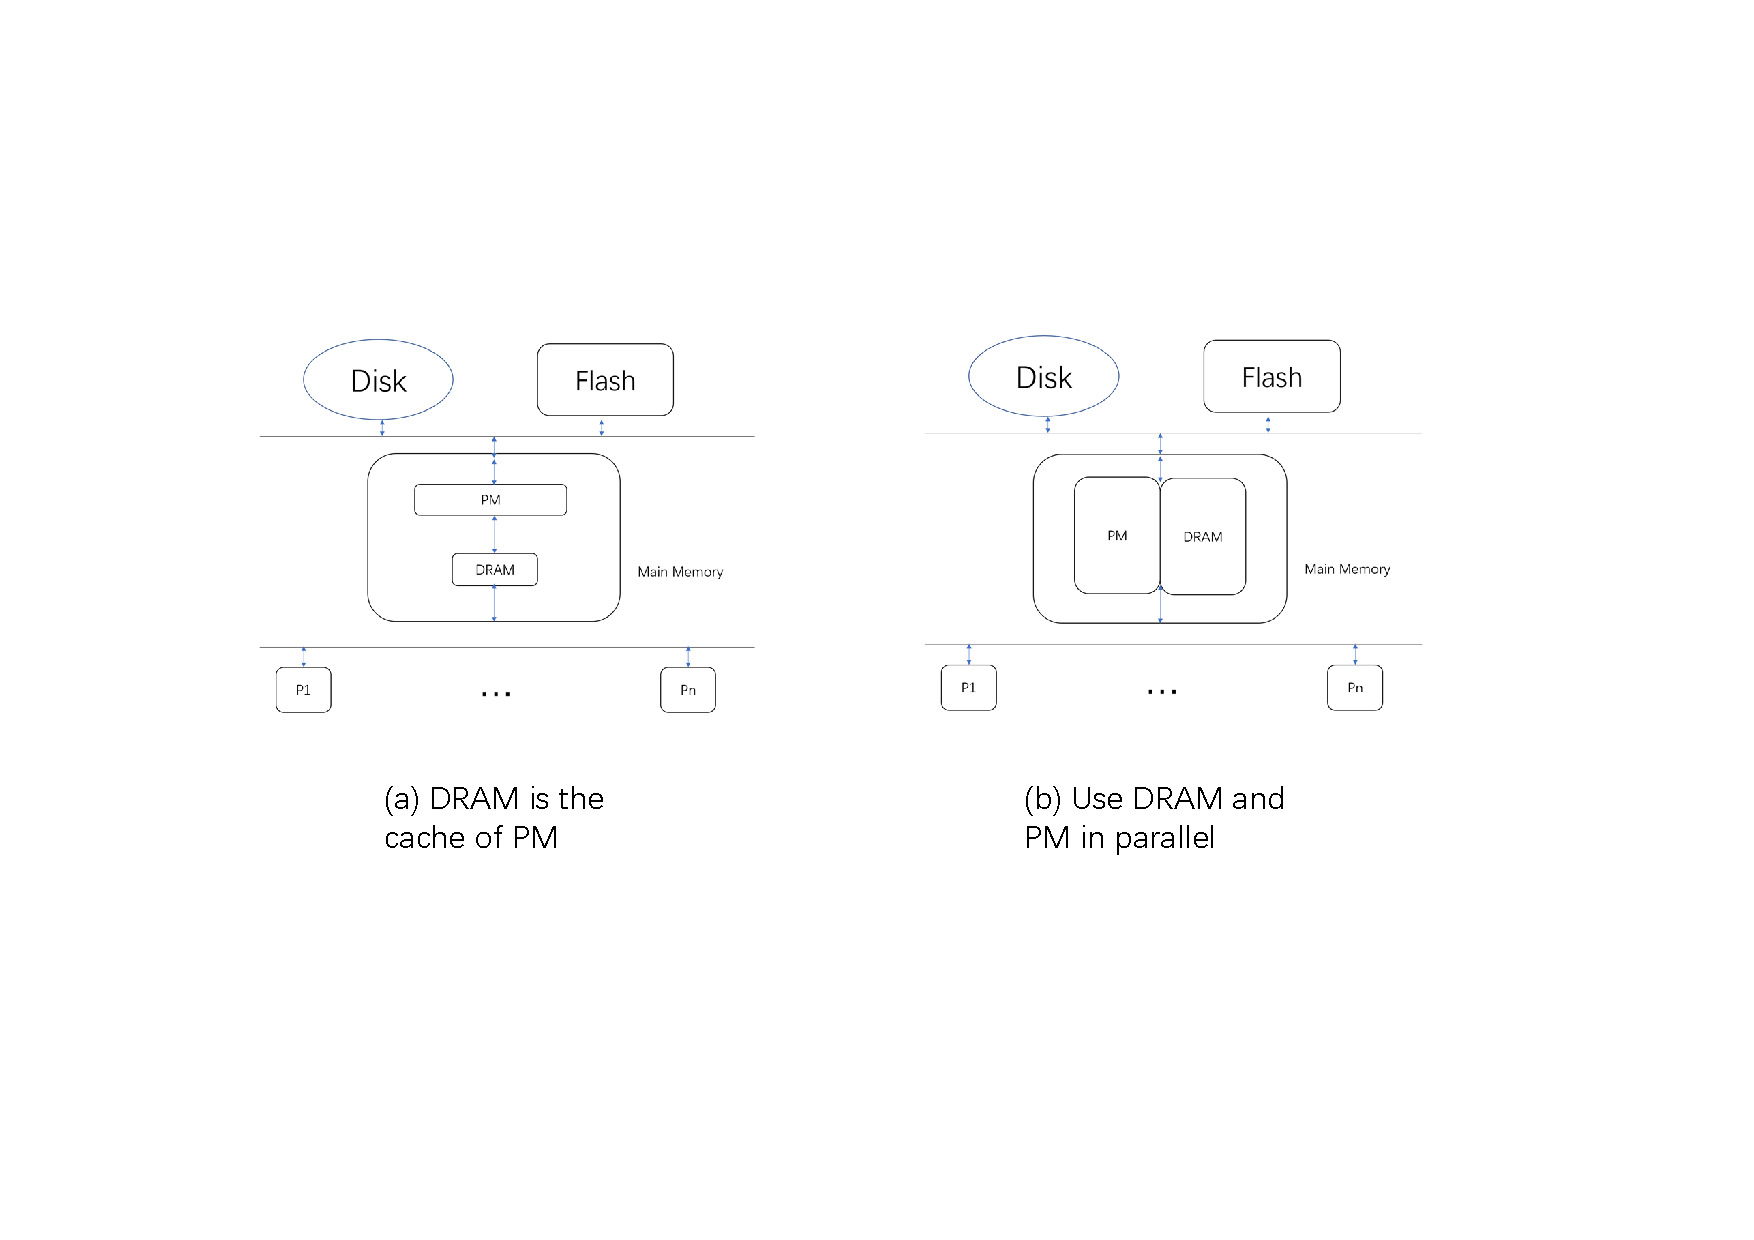
\includegraphics[width=0.36\paperwidth]{figure/PM_DRAM.pdf}
    \caption{Structure of two PM and DRAM mixing methods}
    \label{fig:throughput}
\end{figure}
Take Intel OPTANE DC Persistent Memory\cite{OPTANE} as an example. OPTANE DC Persistent Memory offers two mode: Memory mode and App Direct Mode. When configured to memory mode, application and system sense volatile memory pools. DRAM is used to cache the most frequently accessed data, as well as the PM. It is the first way to mix PM and DRAM. When the App Direct Mode is configured, the application and the operating system clearly know that there are two types of load / storage memory in the platform, and which type of data read / write is suitable for DRAM or Intel OPTANE DC Persistent Memory. Using App Direct Mode, we can store the outstanding transaction version in the DRAM, and use PM to store the MemTable and Immutable MemTable.

Figure 4 shows the algorithm of the Optimistic Concurrency Control of RocksDB. During the commit phase, RocksDB validates the sequence number of each record in the read set. If the latest version of the record does not match the version at the time the record was read, the transaction will abort. There is an observation to introduce the DRAM-based cache: during the commit phase, if the latest version has been flushed into the SSTable, we have to retrieve the record in the SSTable, which will affect the performance due to read amplification. In RocksDB, it maintains the minimal sequence number in the memory, and gets the global sequence number when reading a record. When validating, if the earliest sequence number is smaller than the global sequence number, we only need to validate the version in memory. This approach has some weakness. It will abort some transactions which are legal when the record version has been flushed into the SSTable. There are many approaches to solve this problem. For example, we can attach an index to each record flushed to the disk, but the index will occupy much memory space, which DRAM can't afford. In the OCC optimization, in order to reduce the memory footprint, we do not create an index for each record. What we are concerned with is only the outstanding transaction version, so we can just cache the outstanding transaction version. In PC-DB, DRAM is introduced as the cache. We use the map data structure to store the outstanding transaction version, and we use the App Direct Mode of the Intel OPTANE DC Persistent Memory to store the map in the DRAM. After PC-DB commits a transaction, it should update or add the corresponding records` versions in the DRAM. 
We use DRAM to store the oustanding transaction versions, but there is another problem when validating the version in the validation phase of OCC: when validating, whether PC-DB should first search the DRAM for the lastest version of records, or it should first search the PM for the version? If the PC-DB first search the DRAM for the lastrst version, we should make sure the version of the records in the DRAM must be the latest all the time. In such a situation, when a transaction want to commit, it should first insert or update the version of the records in the DRAM, and then commit itself.In this period, it should get a lock to avoid other transactions update the versions of the record in the meanwhile. Also, to avoid the transaction is aborted after it update the versions of the records and before it commit itself, PC-DB should keep the log, and recover the version in the DRAM based on the log when the transaction is aborted at this time. The lock and the log will be the performance bottleneck if there are many transactions racing in the system. Thus, the validation strategy of the OCC in PC-DB is: to validate the version in the read set during the commit phase in OCC, when the version cannot be retrieved in the persistent memory, PC-DB will retrieve  the key in the  DRAM-based cache and obtain the corresponding version if the key exists in the DRAM. However, if the key is not in the DRAM, PC-DB will set the transaction retry after a period of time, and use a background thread to fetch the lasted version of the key from the disk, rather than just abort the transaction. 
\begin{figure}
    \centering
    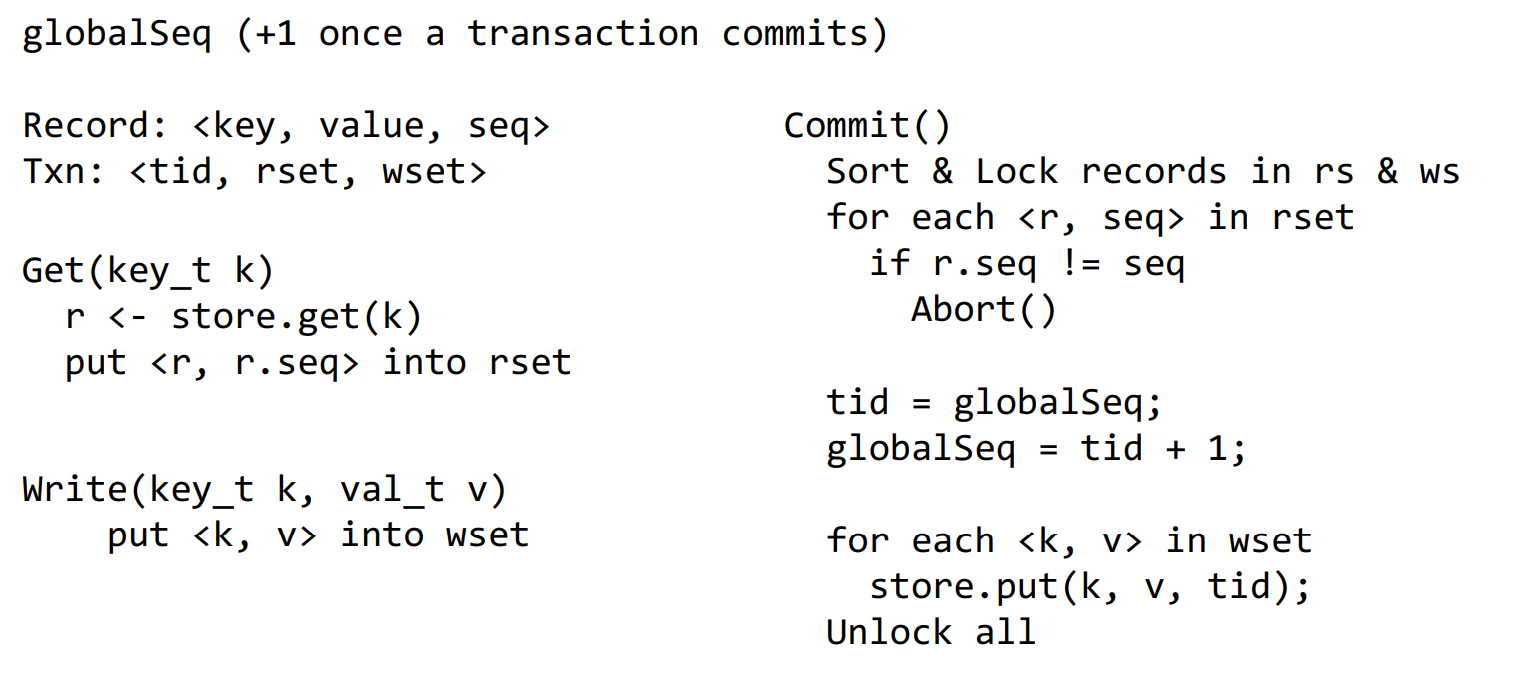
\includegraphics[width=0.36\paperwidth]{figure/algorithm.png}
    \caption{Algorithm of the Optimistic Concurrency Control}
    \label{fig:OCCValidation}
\end{figure}